\documentclass[tikz,border=6pt]{standalone}
\usetikzlibrary{decorations.pathreplacing}

\begin{document}

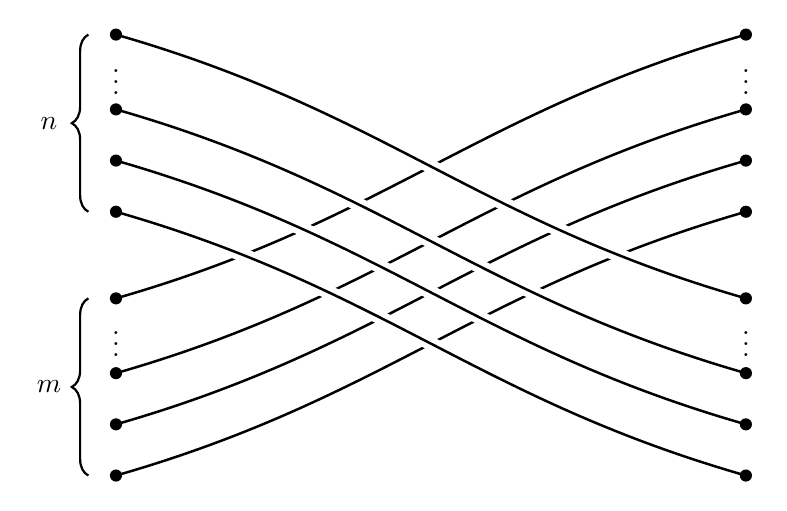
\begin{tikzpicture}[
    strand/.style={
        line width=0.9pt,
        line cap=round,
        line join=round
    },
    overstrand/.style={
        strand,
        preaction={draw=white,line width=5pt,line cap=round}
    },
    dot/.style={circle,fill,inner sep=1.55pt},
    leftbrace/.style={
        decorate,
        decoration={brace,amplitude=6pt},
        line width=0.8pt
    }
]

% ------------------------------------------------
% Geometry: rotated version of the braid
% ------------------------------------------------
\def\xL{0}
\def\xR{8}

% left side: lower block m, upper block n
\coordinate (Lm1) at (\xL,0);
\coordinate (Lm2) at (\xL,0.65);
\coordinate (Lm3) at (\xL,1.30);
\coordinate (Lm4) at (\xL,2.25);

\coordinate (Ln1) at (\xL,3.35);
\coordinate (Ln2) at (\xL,4.00);
\coordinate (Ln3) at (\xL,4.65);
\coordinate (Ln4) at (\xL,5.60);

% right side
\coordinate (Rm1) at (\xR,0);
\coordinate (Rm2) at (\xR,0.65);
\coordinate (Rm3) at (\xR,1.30);
\coordinate (Rm4) at (\xR,2.25);

\coordinate (Rn1) at (\xR,3.35);
\coordinate (Rn2) at (\xR,4.00);
\coordinate (Rn3) at (\xR,4.65);
\coordinate (Rn4) at (\xR,5.60);

% ------------------------------------------------
% Smooth strands
% One family is drawn first; the other is drawn over it.
% ------------------------------------------------

% under family: m on the left to n on the right
\draw[strand] (Lm1) to[out=16,in=196,looseness=1.05] (Rn1);
\draw[strand] (Lm2) to[out=16,in=196,looseness=1.05] (Rn2);
\draw[strand] (Lm3) to[out=16,in=196,looseness=1.05] (Rn3);
\draw[strand] (Lm4) to[out=16,in=196,looseness=1.05] (Rn4);

% over family: n on the left to m on the right
\draw[overstrand] (Ln1) to[out=-16,in=164,looseness=1.05] (Rm1);
\draw[overstrand] (Ln2) to[out=-16,in=164,looseness=1.05] (Rm2);
\draw[overstrand] (Ln3) to[out=-16,in=164,looseness=1.05] (Rm3);
\draw[overstrand] (Ln4) to[out=-16,in=164,looseness=1.05] (Rm4);

% ------------------------------------------------
% Endpoint dots
% ------------------------------------------------
\foreach \P in {Lm1,Lm2,Lm3,Lm4,Ln1,Ln2,Ln3,Ln4,Rm1,Rm2,Rm3,Rm4,Rn1,Rn2,Rn3,Rn4}
    \node[dot] at (\P) {};

% ------------------------------------------------
% Left curly braces and labels
% ------------------------------------------------
\draw[leftbrace] (-0.35,0) -- (-0.35,2.25)
    node[midway,xshift=-0.5cm] {$m$};

\draw[leftbrace] (-0.35,3.35) -- (-0.35,5.60)
    node[midway,xshift=-0.5cm] {$n$};

% ------------------------------------------------
% Ellipses indicating omitted strands
% ------------------------------------------------
\node at (\xL,1.78) {$\vdots$};
\node at (\xL,5.10) {$\vdots$};

\node at (\xR,1.78) {$\vdots$};
\node at (\xR,5.10) {$\vdots$};

% \node at (2.2,2.2) {$\vdots$};
% \node at (2.2,3.4) {$\vdots$};

\end{tikzpicture}

\end{document}